\documentclass[tikz, border=10pt]{standalone}

\usepackage{tikz}
\usetikzlibrary{arrows, intersections}

\tikzset{
    dot/.style = {draw, fill=white, circle, inner sep=0pt, minimum size=4pt},
    >=stealth',
    shorten >=0.5pt, shorten <=0.5pt    
}

\begin{document}
    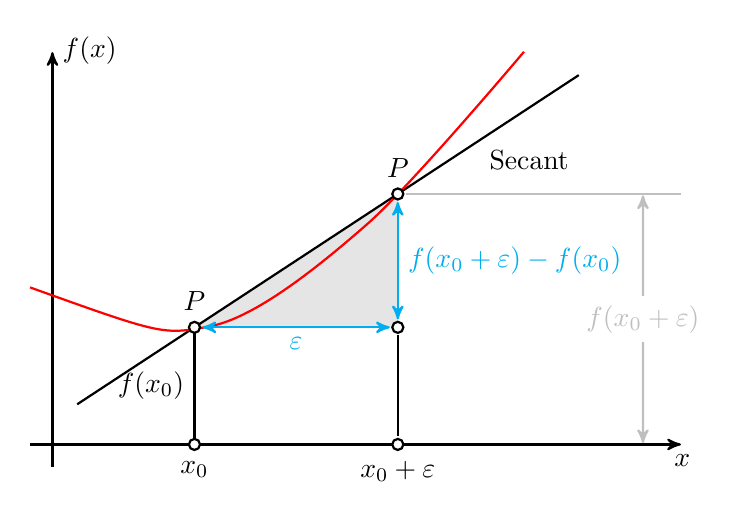
\begin{tikzpicture}[thick]
        \coordinate (O) at (0, 0);
        \path[draw, ->] (-0.3, 0) -- (8, 0) node[below] (xmax) {$x$};
        \path[draw, ->] (0, -0.3) -- (0, 5) node[right] (ymax) {$f(x)$};
        \path[name path=x] (0.3, 0.5) -- (6.7, 4.7);
        \path[name path=y] plot[smooth] coordinates {(-0.3,2) (2,1.5) (4,2.8) (6,5)};
        \scope[name intersections={of=x and y, name=i}]
            \path[fill=gray!20] (i-1) -- (i-2) -- (i-2 |- i-1) -- cycle;
            \path[draw] (0.3, 0.5) -- (6.7, 4.7) node[pos=0.8, below right] {Secant};
            \path[draw, red] plot[smooth] coordinates {(-0.3,2) (2,1.5) (4,2.8) (6,5)};
            \path[draw] (i-1) node[dot, label={above:$P$}] (i-1) {} -- node[left] {$f(x_0)$} (i-1 |- O) node[dot, label={below:$x_0$}] {};
            \path (i-2) node[dot, label={above:$P$}] (i-2) {} (i-2 |- i-1) node[dot] (i-12) {} (i-2 |- O) node[dot, label={below:$x_0 + \varepsilon$}] (i-20) {};
            \path[draw, <->, cyan] (i-1) -- node[below] {$\varepsilon$} (i-12);
            \path[draw, <->, cyan] (i-2) -- node[right] {$f(x_0 + \varepsilon) - f(x_0)$} (i-12);
            \path[draw] (i-12) -- (i-20);
            \path[draw, gray!50] (i-2) -- (i-2 -| xmax);
            \path[draw, <->, gray!50] ([xshift=-0.5cm]i-2 -| xmax) -- node[fill=white] {$f(x_0 + \varepsilon)$} (7.5cm, 0cm);
        \endscope
    \end{tikzpicture}
\end{document}